% ! TeX root = ../../main.tex
\chapter{Implementazione}
In questo capitolo vengono trattate le implementazioni e i pattern utilizzati per raggiungere i requisiti di progettazione presentati nel capitolo precedente. Sono presentate le effettive schermate ottenute partendo dai mockup mostrandone porzioni di codice particolarmente interessanti o dove sono stati applicati pattern.

I sorgenti del progetto sono organizzati in cartelle relative a ciascuna schermata, componente o funzionalità. L'albero delle cartelle del progetto del totem, chiamato TotemBoschettoAR \cite{repoTotemBoschettoAR}, viene presentato nel listato \ref{lst:projectDir} dove vengono espanse solo le cartelle di primo livello (model, views e dataProvider). All'interno della cartella \texttt{model} sono state inserite le classi che definiscono il modello dei dati utente (file \texttt{share\_data\_model.dart}) e i metodi/classi/interfacce di utilità (file \texttt{obj2map.dart}), in \texttt{views} sono presenti i file delle schermate raccolti in cartelle e infine in \texttt{dataProvider} sono contenuti tutti i provider di dati con cui comunica il \texttt{DataManager} (file \texttt{data\_manager.dart}).

\begin{lstlisting}[language=C, caption={Albero della directory del progetto TotemBoschettoAR}, label={lst:projectDir}]
    TotemBoschettoAR/
        |
        +- model/
            |
            +- obj2map.dart
            +- share_data_model.dart
        +- views/
            |
            +- common/
            +- navigation_menu/
            +- home_page/
            +- stats_page/
            +- chart_page/
            +- info_page/
            +- home_page.dart
            +- stats_page.dart
            +- chart_page.dart
            +- info_page.dart
        +- dataProvider/
            |
            +- firebase_provider.dart
        +- unit_converter.dart
        +- data_manager.dart
        +- main.dart
\end{lstlisting}
% Lavorando in Flutter e dart ciascuna schermata è una composizione di widget

\section{App Mobile}
Seguendo i mockup sono state sviluppate le diverse schermate per la condivisione dei progressi. Sono state effettuate alcune modifiche come si può notare dagli screenshot in figura \ref{fig:shareDataApp}: invece del nickname utente viene indicato come visualizzare il QR code sul totem che nel mockup veniva mostrato invece nella pagina di scansione, infine nella schermata di caricamento è stata modificata sostituendo l'icona e mostrando un testo che informi l'utente del caricamento dei dati.
\begin{figure}[h]
    \centering
    \subfloat[Pagina di condivisone progressi]{
        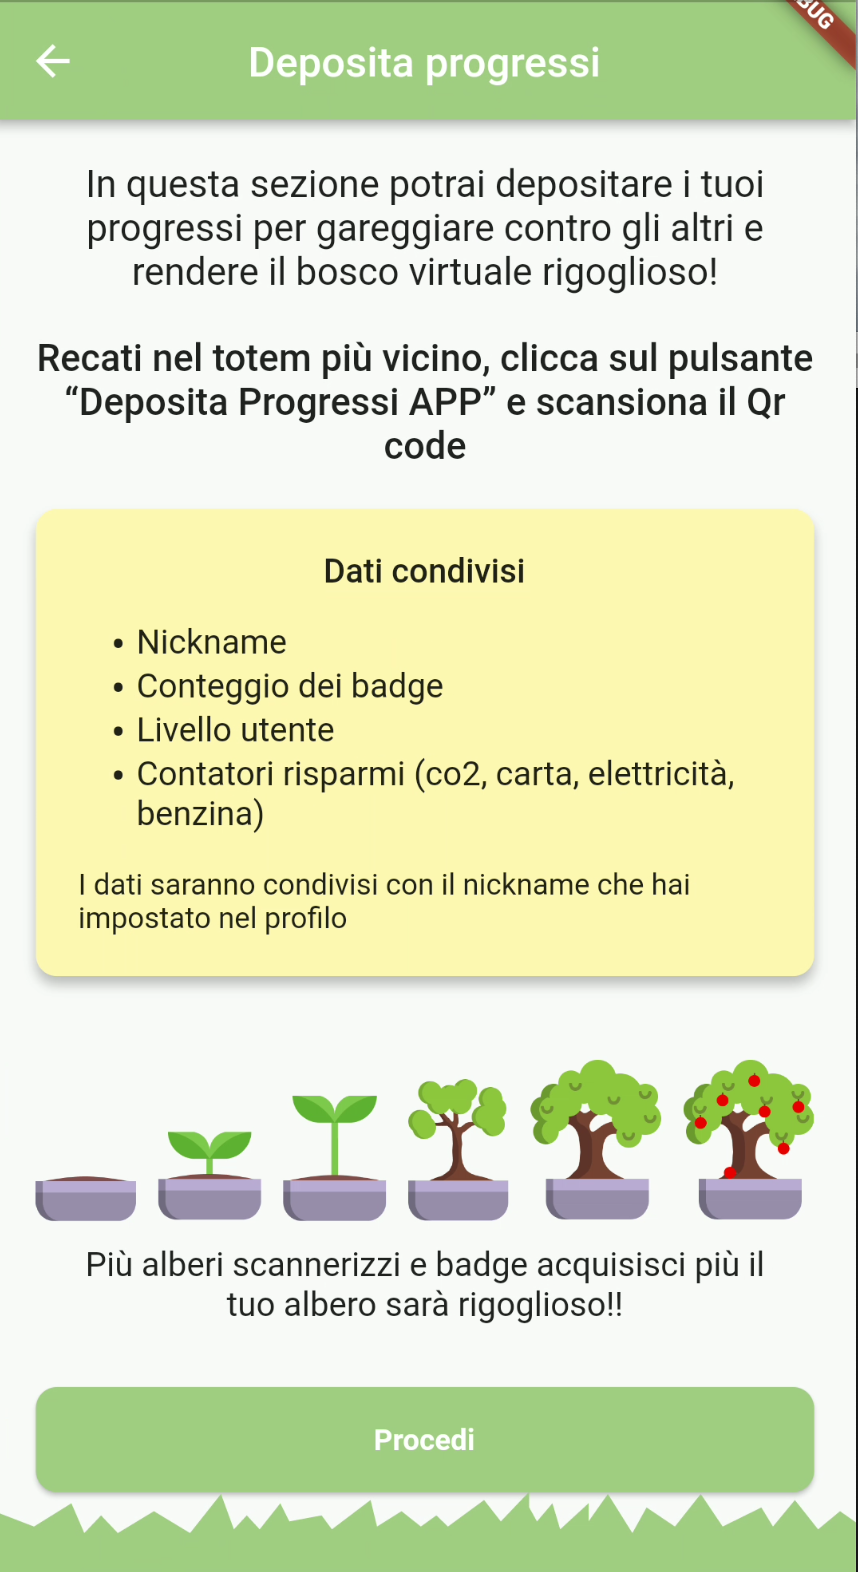
\includegraphics[width=0.3\textwidth]{img/app/uploadPage.png}
        \label{fig:sharePage}
    }
    \subfloat[Scansione QR code totem]{
        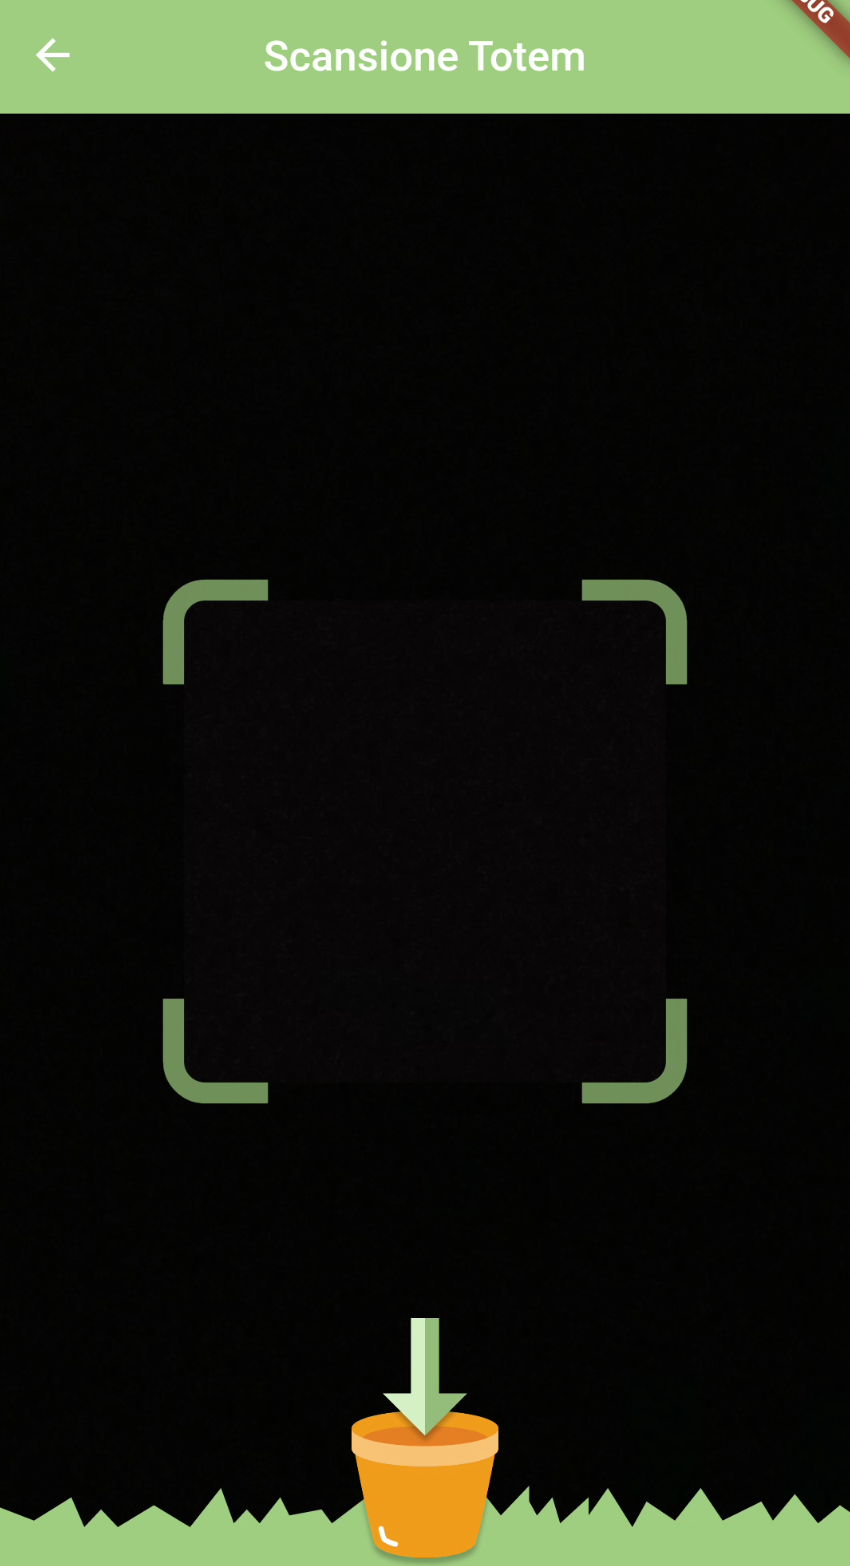
\includegraphics[width=0.3\textwidth]{img/app/uploadProgress.png}
        \label{fig:scanTotem}
    }
    \subfloat[Schermata di caricamento progressi]{
        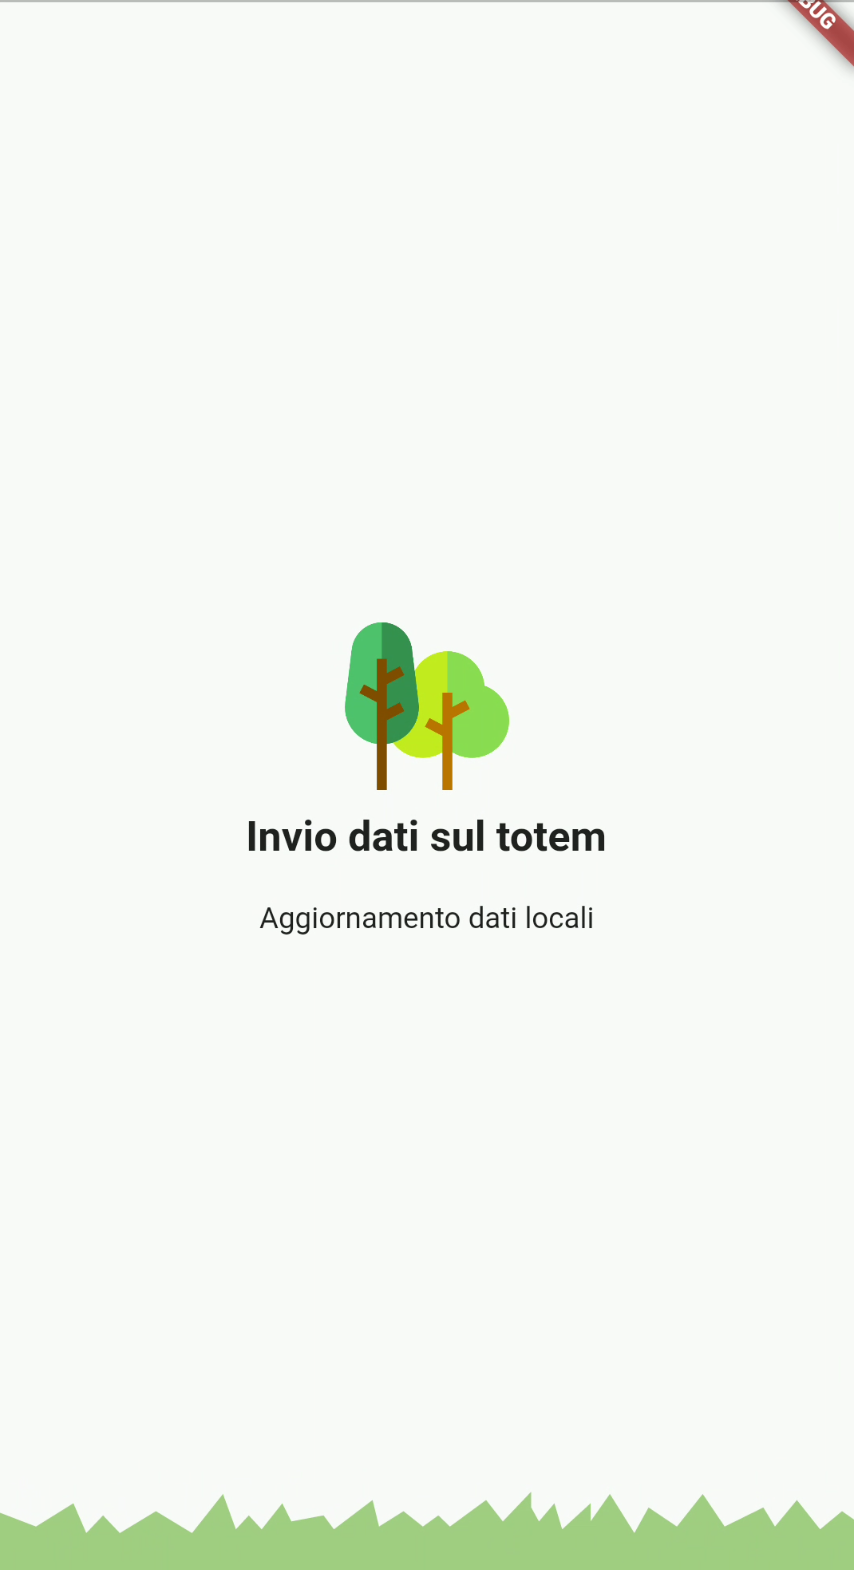
\includegraphics[width=0.3\textwidth]{img/app/uploadingPage.png}
        \label{fig:uploadinData}
    }
    \caption{Schermata condivisione dati da app}
    \label{fig:shareDataApp}
\end{figure}

Questa schermata è raggiungibile dalla pagina utente oppure direttamente dalla pagina \textit{Home} in cui vi sono gli alberi collezionati. In entrambe le pagine è stato aggiunto all'AppBar il pulsante \texttt{IconButton} che inserisce la schermata allo stack di navigazione. Nel listato \ref{lst:shareIconButton} viene mostrato il codice inserito

\begin{lstlisting}[style=FlutterStyle, caption=Python example, label={lst:shareIconButton}]
    Scaffold (
      backgroundColor: Colors.white,
      appBar: AppBar(
        centerTitle: true,
        backgroundColor: mainColor,
        title: const Text("Profilo"),
        leading: IconButton(
          onPressed: () => Navigator.push(
            context,
            MaterialPageRoute(builder: (context) {
              return const SharePorgressPage();
            }),
          ),
          icon: const Icon(
            Icons.upload,
            size: 25,
            semanticLabel: "Carica progressi",
          ),
        ),
      ),
      body: //contenuto della pagina Utente o della Home
    );
\end{lstlisting}
% Implementazione della sch rmata di scansione del qr del riutilizzo della schermata di scansione (forze pattern strategy), con schema d'interfaccia volendo 
% Implementazione della schermata con codice effettivo dell'implementazione del pattern mvi


\section{Totem}
\subsection{Dati Firebase}
% Come sono stati modellati i dati caricati su un totem su Firebase, struttura generale dei dati JSON ed esempio
% regole di accesso al database

Avendo deciso di utilizzare il database Firebase Realtime, che è di tipo documentale, si è reso necessario convertire lo schema UML in figura \ref{fig:totemDomain} in formato JSON per avere la struttura generale dei dati che verranno memorizzati.
Per non avere troppi oggetti annidati, si è deciso di separare le informazioni del totem (listato \ref{lst:totemInfo}) dai dati utente che sono stati condivisi (listato \ref{lst:userDataTotem}).

\begin{lstlisting}[language=json, caption={}, label={lst:totemInfo}]
    "totemInfo": {
        "totemIdString": {
          "place": "locationName",
          "project": "projectName"
        },
      },
\end{lstlisting}  

\begin{lstlisting}[language=json, caption={}, label={lst:userDataTotem}]
      "totems": {
        "ces_remade": {
          "userNickname": {
            "badgeCount": 0,
            "co2": 0,
            "level": 0,
            "nickname": "userNickname",
            "paper": 0,
            "treesCount": 0
          }
        }
      }
\end{lstlisting}

\subsection{Datamanager}
%Come è il datamanager, cosa ritorna e come viene gestito il pattern observer di Firebase che chiama metodo dopo che il db viene modificato
Il data manager, come spiegato nel capitolo del design, funge da repository e da Model nel pattern MVI.
Al suo interno mantiene un riferimento al database firebase...



\subsection{statspage}
Animazione dell'elemento della griglia, creazione della pagina, quali widget flutter sono stati utilizzati e codice di pattern mvi per il caricamento dei dati e la loro attesa, operazioni che vengono svolte all'interno di data manager per ricavare i dati
\subsection{Classifica}
Schermata della classifica, le modifiche grafiche che ha subito, l'aggiunta dell'alberello e info di co2, caricamento dati solito pattern mvi, come viene stilata la classifica codice lato repository (datamanager)... Ipotesi di poter decidere su cosa viene fatta la classifica es. co2, benzina o che altro. anche se poi alla fine le quantità sono proporzionali, cambierebbe poco la classifica.

\subsection{infopage}
Pagina informazioni, struttura a griglia, le classi che sono state create e politica di disposizione delle tiles;  pattern observer per mostrare e chiudere il pop up delle info
come si deve fare per aggiungere una tile e impostazioni delle tile, grandezza e contenuto
